\documentclass[letterpaper,12pt]{article} %amsart
\usepackage[raggedright]{titlesec}
\usepackage[margin=1in]{geometry}
%\renewcommand{\thesection}{\Large{\textbf{section}}}
%\renewcommand{\thesubsection}{\Alph{subsection}}
\usepackage{indentfirst}
\usepackage{secdot}
\usepackage{titlesec}
\usepackage{xcolor, soul}
\usepackage{mathabx}
\usepackage{enumitem}
\usepackage{times}
\usepackage{float}
\usepackage{parcolumns}


\usepackage{listings}
\usepackage{xcolor}

\definecolor{codegreen}{rgb}{0,0.6,0}
\definecolor{codegray}{rgb}{0.5,0.5,0.5}
\definecolor{codepurple}{rgb}{0.58,0,0.82}
\definecolor{backcolour}{rgb}{0.95,0.95,0.92}

\lstdefinestyle{mystyle}{
    backgroundcolor=\color{backcolour},   
    commentstyle=\color{codegreen},
    keywordstyle=\color{magenta},
    numberstyle=\tiny\color{codegray},
    stringstyle=\color{codepurple},
    basicstyle=\ttfamily\footnotesize,
    breakatwhitespace=false,         
    breaklines=true,                 
    captionpos=b,                    
    keepspaces=true,                 
    numbers=left,                    
    numbersep=2pt,                  
    showspaces=false,                
    showstringspaces=false,
    showtabs=false,                  
    tabsize=4,
    xleftmargin=2cm,
    xrightmargin=2cm
}
\lstset{style=mystyle}
\usepackage{graphicx}
\graphicspath{ {./img/} }
\sethlcolor{yellow}
\sectiondot{subsection}
\setlength{\parindent}{1em}
\raggedbottom %*fix for extra gap between paragraphs in ML section

\iffalse
\makeatletter
\def\specialsection{\@startsection{section}{1}%
  \z@{\linespacing\@plus\linespacing}{.5\linespacing}%
%  {\normalfont\centering}}% DELETED
  {\normalfont}}% NEW
\def\section{\@startsection{section}{1}%
  \z@{.7\linespacing\@plus\linespacing}{.5\linespacing}%
%  {\normalfont\scshape\centering}}% DELETED
  {\normalfont\scshape}}% NEW
\makeatother
\fi


\titleformat{\section}{\centering\uppercase}{\thesection.}{0.5em}{}
\titleformat{\subsection}{\itshape}{\thesubsection.}{0.5em}{}

\renewenvironment{abstract}{\textbf{\textit{Abstract---}}}{}

\begin{document}
\title{\Large{\textbf{OpenMP for Python Technical Overview}}}
\author{Caleb Huck}
\date{June 3rd, 2021 ************ change}
\maketitle
%\clearpage

\section{Overview}
OpenMP for Python is currently a prototype level software that brings core OpenMP function and behavior to the Python language. It is designated as a prototype because the goal of this project, to this point, was to implement a proof-of-concept that not only could OpenMP be adapted to the Python syntax and paradigm in a way that is intuitive and usable, but that parallel concepts (e.g. concurrency, speedup, efficiency, etc.) could be demonstrated clearly for the specific purpose of teaching. While performance is something we care about, in the context of demonstrating the benefits of parallelism, it is not our goal to provide a real world performance tool, as real world performance applications would always benefit from using a more appropriate language. To that end, we have kept the design as simple as possible in order to quickly realize our proof-of-concept and provide a base that can be continually developed in the future into a robust tool for teaching. 

This software currently includes a specific subset of the full OpenMP specification. We have deliberately selected specific directives, clauses, and runtime functions that represent the core functionality needed to implement most any parallel algorithm. This subset of the full standard is sufficient for our needs but can easily be added to in the future if needed. It is important to note that, while it was our goal for the current implementation to follow the OpenMP standard as closely as possible at this time, it is still not ``one-to-one" with OpenMP. There are likely still corner cases where the behavior of our software will differ with OpenMP. We have made an effort to test each construct during development to catch as many inconsistencies as possible, however, it will take significant user testing and iterative improvement in the future to fully capture OpenMP behavior, at least to the degree that it is possible. Additionally, there are some differences between our software and original OpenMP that are a result of the inherent differences between C-like languages and Python. This is inevitable given the many paradigmatic incongruencies between these languages. 

This document provides a general overview of the design, architecture, and implementation of this software. Our goal is to provide background on the technical aspects of the project, explain the functional design and software architecture, and finally, demonstrate results from our microbenchmarks and cover some of the interesting points regarding them. It is our intention to give the most comprehensive technical understanding of our software possible without being overly verbose. Finally, the user API will not be included in this document. Instead, it will be provided in a separate user document.  \hl{The organization of this document is as follows: the next section will give a high-level functional overview of the software architecture and its components, followed by a brief explanation of how data flows through the application. }

\section{Architecture Overview}
The basic flow of the application is shown in figure \ref{fig:arch_flow}. The large arrows represent the flow of the source code through the software and the small arrows denote communication that doesn't involve the source code. We use a modified version of the Jython interpreter since it does not implement a Global Interpreter Lock like CPython and therefore is able to run multithreaded code truly in parallel, using the underlying Java threads (Jython is written in Java). Currently, our OpenMP source-to-source preprocessor is written in Python. The reason for this is that Python was an easy choice early on for quick prototyping and testing Python code transformation before we had made a commitment in terms of design and project direction. If we had been sure about our approach using Jython from the beginning, we likely would have written the preprocessor in Java in order to have a more seamless integration between interpreter and preprocessor.  Nonetheless, our current, more separated approach allows for flexibility in the future if we want to use our preprocessor with a different interpreter. Additionally, porting our solution to Java would also be a straightforward task if desired since our parser generator (ANTLR4) can easily be used with Python or Java.

Since our preprocessor is written in Python, it runs in a separate process than the interpreter. We accomplish this by spawing a subprocess using the Java ProcessBuilder class. This allows us to start the preprocessor, passing in the fully qualified path to the source code file as a command line argument to the python process, and finally capturing the output (whether it be the transformed source code, or an error output). 

The preprocessor consists of two main components: the ANTLR lexer/parser (which are automatically generated by ANTLR from our modified Python grammar file), and the Translator Visitor. The Translator Visitor traverses the abstract syntax tree produced by the parser and is responsible for creating the multithreaded code that will run on Jython. The visitor object contains one visitor function per rule from the grammar that is  triggered every time that rule is encountered. If it is rule pertaining to regular Python statements, then the visitor just ``prints" the code with no changes. But if the rule pertains to an OpenMP statement, then the visitor function instead prints the  multithreaded equivalent of the OpenMP code. \hl{Exactly how the code is transformed will be covered in more detail later.} At this point, if no errors were generated during the lexing/parsing, the new source code is printed to stdout, where it is then captured by Jython and written to a temporary file. In contrast, if an error was generated, only the error is printed and will be displayed to the user from Jython before exiting with an error status.  

Lastly, some of the output code, such as OpenMP for loops, require runtime calls to be made. For example, if the schedule is dynamic, then each thread must make a call to request the next block each time it finishes an assigned block. This is accomplished using the backend runtime, which is not user-visible. In contrast, the omp runtime contains OpenMP API function calls (e.g. $omp\_get\_thread\_num()$ and $omp\_get\_num\_threads()$), and is user visible. Both of these modules reside in a directory within the preprocessor file structure which is added to the path automatically during code transformation. \hl{check how user imports ompy after benchark finishes}.  

\begin{figure} [H]
    \centering
          {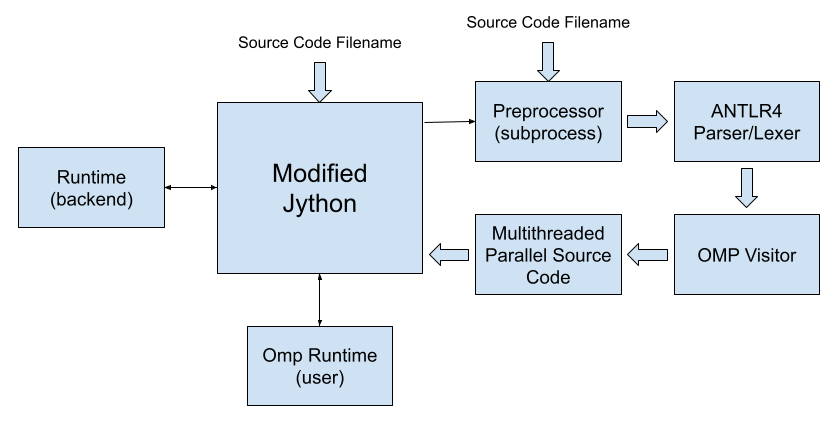
\includegraphics[width=.8\textwidth]{architecture_flow.png}}
        \caption{HPC Processor Trends Over Time}
        \label{fig:arch_flow}
    \centering
\end{figure}


\section{Code Transformation}
This section gives insight into how the code is transformed from OpenMP blocks to multithreaded code and the strategy behind the preprocessor. Because of some helpful features in the Python language, we are able to translate the code in a single pass using the visitor design pattern. More specifically, nesting parallel function target declarations and variable closures allow us to write the code in the order it is traversed by the visitor because scoping and nesting are handled automatically and don't need special effort to track. lst \ref{lst:ex_1_orig}


\begin{lstlisting}[language=Python, caption={Original Code}, label={lst:ex_1_orig}]{Name}
var = 0
#omp parallel shared(var)
    print(var)
\end{lstlisting}


\begin{lstlisting}[language=Python, caption={Transformed Code}, label={lst:ex_1_trans}]{Name}
_num_threads_ = 1
var = 0
_num_threads_ = 8
def _target_0(_manager_):
    global var
    print var
_manager_outer_ = RuntimeManager(_num_threads_)
submit(_target_0, _num_threads_, args=(_manager_outer_,))
\end{lstlisting}






\end{document}





























